\chapter{Realisierung}

Im folgenden Abschnitt soll auf die Implementierung des \textit{Smart Warehouse} Szenarios eingegangen werden. Insbesondere werden Probleme während der Umsetzung der beiden Objektdetektoren \textit{SSD} und \textit{YOLO} betrachtet, die Realisierung der Dashboard-Webapplikation und des Zählalgorithmus zur Durchführung der Inventur aufgezeigt und letztendlich Herausforderungen im Rahmen der Drohnen Anbindung besprochen.

\section{Umsetzung der Objektdetektoren}

\subsection*{SSD}

Die verwendete Custom-Implementierung in \textit{PyTorch} realisiert die \textit{SSD300} Variante des \textit{SSDs}. Neben kleineren Änderungen in der Codebasis zur Erreichung von Kompatibilität mit aktuellen Bibliotheksversionen und weiteren Anpassungen zur Integration eines eigenen Datenbestandes, wurden vor allem drei größere Erweiterungen durchgeführt. 

Da der erstellte Datenbestand nur 1088 gelabelte Daten enthält, wurde zusätzlich zur Custom-Implementierung ein sechsfaches Kreuzvalidierungsverfahren realisiert, um ein höheres Abstraktionsvermögen des Modells auf dem geringen Datenbestand zu erreichen. Auch unterstützte die Referenzimplementierung keine Validierung durch zuvor ungesehene Daten. Die Modellklassen des Datenbestandes und die Validierungsskripte wurden dahingehend angepasst. Zudem fehlte eine Visualisierung der Entwicklung der Verlustkurven während des Trainingsverfahrens.

Die Referenzimplementierung erstellt sich des Weiteren einige Hilfsdateien, in der die Pfade zu Bildern und weitere Datenstrukturen für Trainingszwecke abgespeichert werden. Ohne diese ist kein Training möglich, das Trainingsskript fordert demnach Zugriff auf den Sekundärspeicher. 

Um ein lokales Training auf der \textit{NVIDIA GeForce GTX 1080} GPU zu ermöglichen, wurde zudem \textit{CUDA} Version 10.1 verwendet. Trainiert wurde mit folgenden Hyperparametern:
\begin{itemize}
	\item Batchgröße: 16
	\item Lernrate: $1.0\cdot 10^{-3}$
	\item Momentum: 0.9
	\item Kreuzvalidierungen: 6 à 22 Epochen
	\item Epochen: 132
	\item Gradientenverfahren: Mini-Batch
	\item Aktivierungsfunktion: ReLU
	\item Kostenfunktion: Smooth L1
\end{itemize}

Das Basisnetzwerk des \textit{SSDs} besteht aus einem auf \textit{ImageNet} vortrainierten \textit{VGG16}. Die restlichen \textit{Convolutional Layer} sind \textit{Xavier} initialisiert. 

Die Hyperparameter sind nahezu gleich zu denen in der ursprünglichen wissenschaftlichen Veröffentlichung. Die Batchgröße im \textit{Mini-Batch} Verfahren wurde für größere Stabilität von 32 auf 16 heruntergesetzt. Auch in der Evaluierung wurde die Batchgröße von 64 auf 48 verkleinert, da die Eingangsdaten eine weitaus höhere Auflösung als die ursprünglich im \textit{PascalVOC} verwendeten Daten haben. Andernfalls wird Gefahr gelaufen, einen Speicherüberlauf zu verursachen. Der Datensatz wurde in fünf Untermengen unterteilt, in jedem Kreuzvalidierungsschritt diente jeweils eine Untermenge als Testdatensatz.

\subsection*{YOLO}

Für \textit{YOLO} wurde die neuste Version \textit{YOLOv3} implementiert. Hierbei kommt das \textit{Dark-""net} Framework zum Einsatz, eine Implementierung in C. Vor der initialen Kompilierung müssen einige Konfigurationsschritte unternommen werden, weil auch der Betrieb auf einer normalen CPU oder einer GPU mit Tensor Kernen möglich ist. Für das Training kommt eine \textit{NVIDIA GeForce RTX 2060} GPU auf Basis von \textit{CUDA} Version 10.0 zum Einsatz, deren enthaltenen Tensor Kerne mitbenutzt werden. Zudem ermöglicht \textit{YOLO} die Nutzung von \textit{cuDNN} Version 7.4 für hardwarebeschleunigte Matrizenoperationen. Die benötigten Hyperparameter wurden dabei wie folgt gesetzt:

\begin{itemize}
	\item Batchgröße: 64
	\item Subdivisions: 16
	\item Lernrate: $1.0\cdot 10^{-3}$
	\item Momentum: 0.9
	\item Maximale Anzahl Batches: 18000
	\item Gradientenverfahren: Mini-Batch
	\item Aktivierungsfunktion: LReLU
	\item Kostenfunktion: Summe der Fehlerquadrate
\end{itemize}

Im Unterschied zum \textit{SSD} kann \textit{YOLO} die in den GPU Speicher zu ladende Datenmenge eines Batches durch sogenannte \textit{Subdivisions} festgelegt. Hierbei werden nur noch $Batchgroesse \div Subdivisions$ Bilder gleichzeitig in die GPU geladen, um einen Speicherüberlauf zu vermeiden.

Die Lernrate sowie das Momentum bleiben wie in der Dokumentation empfohlen unverändert zu den Referenzwerten. Im Gegensatz zu \textit{SSD} wird kein Maximum für die Anzahl an Epochen, sondern ein Maximalwert für die zu durchlaufenen Batches gesetzt. Dieser Wert wird abhängig von der Menge an gelabelten Klassen gesetzt und kann als Empfehlung aus der Dokumentation für das \textit{Darknet} Framework entnommen werden. 

\section{Dashboard Entwicklung}

Der Server wurde mit dem \textit{Flask} Framework in Python implementiert und läuft auf dem \textit{Web Server Gateway Interface} (WSGI) server \textit{Waitress}. Er führt den Inferenzalgorithmus des \textit{SSDs} bzw. des \textit{YOLO} Objektdetektors für jeden Frame des empfangenen Videostreams der Drohne aus und streamt die inferierten Bilder mit den Bounding Boxen an jeden Client. Der Client wurde mit dem \textit{Bootstrap} Framework grafisch gestaltet (siehe Abbildung \ref{webapp}).

\begin{figure}[H]
	\begin{center}
		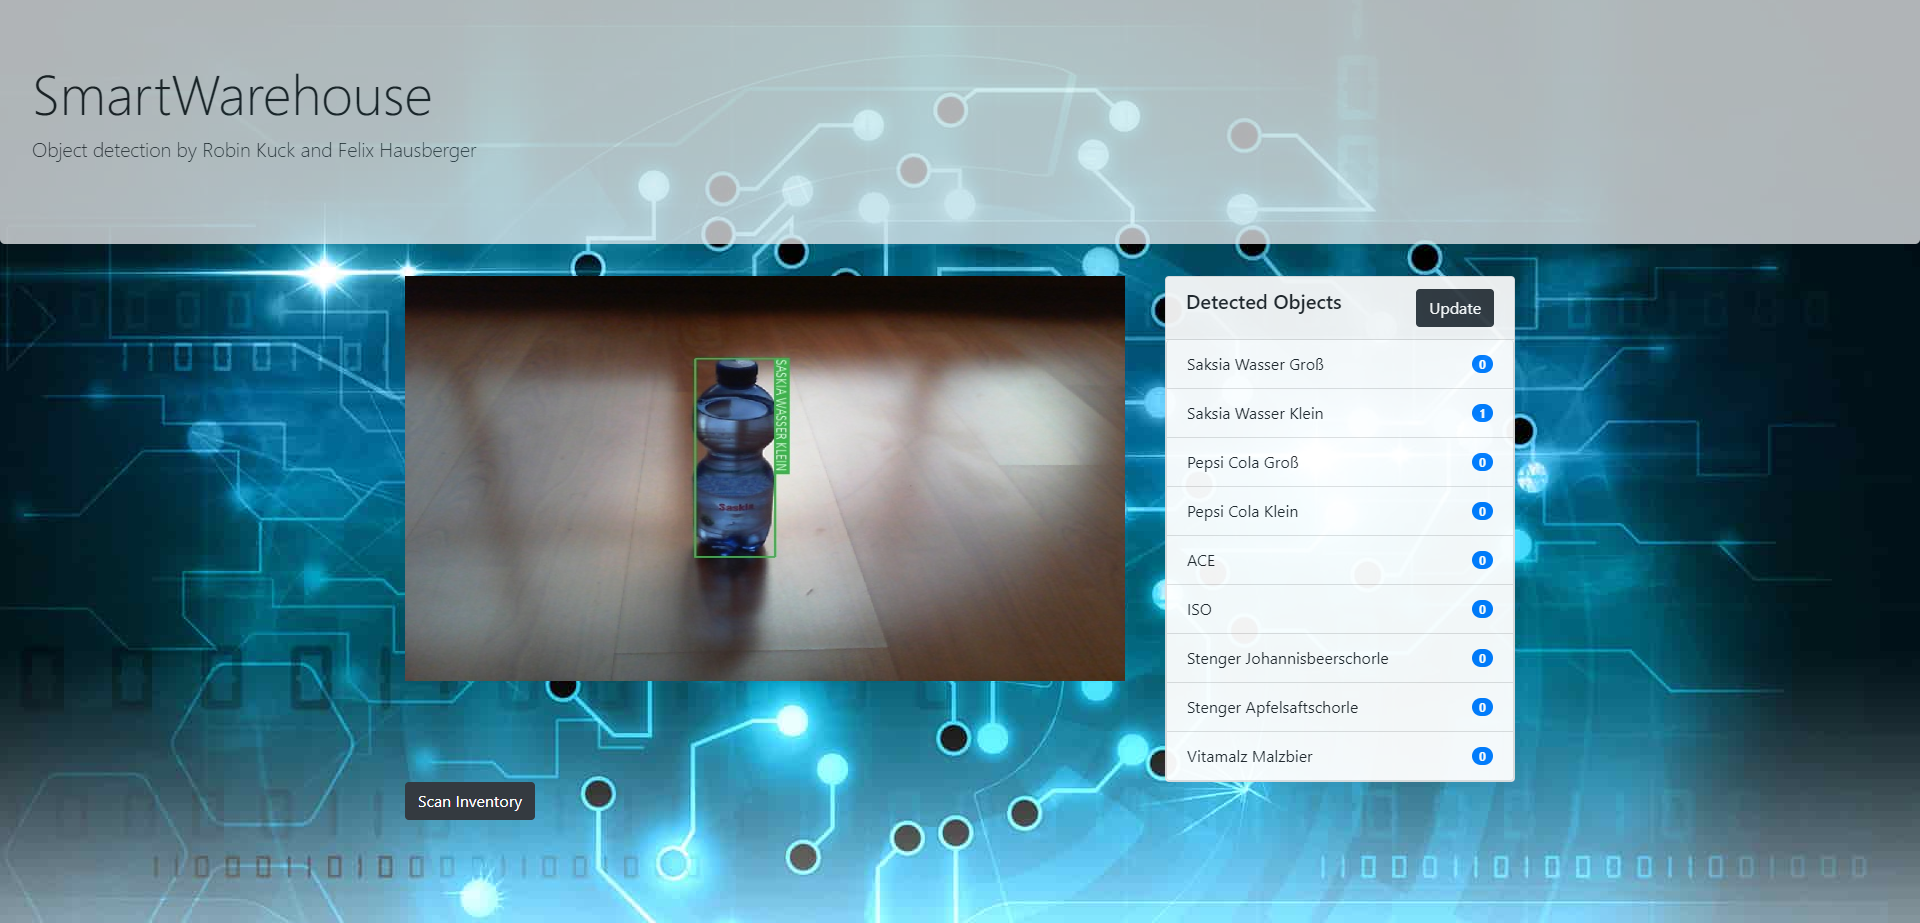
\includegraphics[width=15cm]{Bilder/webapp.jpeg} 
		\caption[Webapplikation Smart Warehouse]{Webapplikation Smart Warehouse}
		\label{webapp}
	\end{center}
\end{figure}

Auf Anfrage eines Client kann dieser die aktuell gezählten Objekte vom Server abfragen. Der Zählalgorithmus wird im folgenden Unterkapitel erklärt. 

\section{Zählalgorithmus}

\lstinputlisting[
label={code:formfield},
caption={Zählalgorithmus zum Zählen der detektierten Objekte},
captionpos=b,
basicstyle=\ttfamily\scriptsize,   
firstline=1,              
lastline=11                 
]{Quellcode/algorithmus.txt}

Der Algorithmus \ref{code:formfield} wird momentan dazu verwendet, um für das Industrieszenario einer Inventur einzelne detektierte Objekte zu zählen. Nach jedem Inferenzvorgang werden die detektierten Objekte abgespeichert, sodass der Algorithmus bei Aufruf sowohl auf die zuletzt detektierten Objekte \textit{o\_alt}, als auch auf die neu detektierten Objekte \textit{o\_neu} zugreifen kann. Für alle detektierten Objekte im aktuellen Durchlauf durchsucht er alle zuletzt detektierten Objekte, um herauszufinden, ob ein Objekt bereits im vorherigen Bild vorhanden war. Ausschlaggebend hierfür ist das gleiche \textit{Label} als auch die Distanz der Bounding Boxen des aktuell detektierten Objekts zum Objekt der Vorrunde. Nur falls das Objekt nach diesen Kriterien nicht bereits in der Vorrunde vorhanden war, wird es gezählt. Das Problem, das der Algorithmus zu lösen versucht, enthält allerdings eine weitere Komplexitätsstufe. Dasselbe Objekt kann im Laufe der Inventur erneut auftreten und dessen relative Position im Bild ist ebenso variabel. In diesem Falle werden Objekte doppelt gezählt. 

\section{Drohnen Anbindung}
Für die Steuerung sowie den Zugriff auf den Videostream bietet die \textit{Tello EDU} ein eigenes WiFi Netz an, zu dem sich das Steuergerät verbinden muss. Die Kommunikation erfolgt über das \textit{UDP} Protokoll\footnote{UDP steht für User Datagram Protocol. Es ist ein Transportprotokoll, welches im Gegensatz zu TCP verbindungslos und nicht zuverlässig ist.} und besteht aus mehreren Kommunikationskanälen. Der Video Stream und der Status der \textit{Tello EDU} werden unidirektional durch die Client Applikation bei der \textit{Tello EDU} abgefragt, wohingegen für das Senden von Befehlen eine separate, bidirektionale Verbindung zum Einsatz kommt. Das liegt daran, dass die \textit{Tello EDU} auf jeden erhaltenen Befehl auch eine Antwort zurücksendet. Es existieren Befehle zur Steuerung und zum Auslesen von Informationen wie zum Beispiel der Geschwindigkeit oder Ladezustand der Batterie. Als Hilfestellung für wird ein Beispielprogramm mitgeliefert, in welchem das Senden und Empfangen von Befehlen implementiert wurde \cite{RyzeTech.2018}. 

\subsection*{Flugsequenz}
Für die Flugsequenz bietet die Kommunikation durch eine Socket\footnote{Mit Sockets können Daten bidirektional zwischen  Programmen ausgetauscht werden, die entweder auf dem gleichen oder auf einem anderen durch eine Netzwerkadresse erreichbaren PC laufen.} Verbindung die ideale Lösung. Python bietet ein \textit{socket} Modul an, welches verschiedene Typen von Sockets unterstützt. Das nachfolgende Listing zeigt die Initialisierung einer Instanz der Socket Klasse:

\lstinputlisting[
label={code:python},
caption={Initialisierung der Socket Klasse},
captionpos=b,
basicstyle=\ttfamily\scriptsize,   
firstline=1,              
lastline=2                 
]{Quellcode/socket_init.py}

Die Methode \textit{socket()} erzeugt eine neue Instanz der Socket Klasse und benötigt zwei Parameter für die Adressfamilie und den Verbindungstyp. \textit{AF\_INET} steht für Internet-Socket-Adresse, die sich aus IP-Adresse und Portnummer zusammensetzt. Der Parameter \textit{SOCK\_DGRAM} gibt an, dass die Socket Verbindung über das UDP-Protokoll aufgebaut wird. Für das Empfangen von Daten wird die Instanz zusätzlich an eine Adresse (hier \textit{localhost:9000}) gebunden.

Im folgenden Listing wird jeweils die Methode zum Senden von Befehlen und Empfangen von Antworten gezeigt:

\lstinputlisting[
label={code:python},
caption={Methode für das Versenden von Befehlen und Empfangen von Antworten},
captionpos=b,
basicstyle=\ttfamily\scriptsize,   
firstline=1,              
lastline=22                 
]{Quellcode/socket_send_command.py}

Die Methode \textit{send\_command()} erhält beim Aufruf den auszuführenden Befehl als Parameter vom Typ \textit{String}. Für jeden Befehl wird eine neue Instanz der Klasse \textit{Stats} in das \textit{log} Array einfügt. Die Klasse \textit{Stats} dient für die Datenhaltung eines gesendeten Befehls und die entweder noch ausstehende oder bereits erfolgte Antwort. Daraufhin wird der Befehl mit Hilfe der Methode \textit{socket.sendto()} an den Socket übermittelt. Dieser erhält neben dem Befehl auch die Zieladresse, die als Tupel bestehend aus IP-Adresse und Port übergeben wird. Im nächsten Schritt wird mittels einer Schleife auf das Erreichen der Antwort gewartet. Dabei wird die seit dem Versand der Nachricht vergangene Zeit berechnet und wenn diese größer als die auf 15 Sekunden festgelegte Konstante \textit{MAX\_TIME\_OUT} ist, gibt die Methode \textit{False} zurück. Sobald jedoch eine Antwort empfangen wurde, kann die Schleife übersprungen und \textit{True} zurückgegeben werden.

Aufgrund der UDP basierten Verbindung ist nicht garantiert, ob und in welcher Reihenfolge Antworten empfangen werden können. Um dem entgegenzuwirken, kommt die Methode \textit{receive\_thread()} zum Einsatz, die in einem parallel laufenden Thread ausgeführt wird und die empfangene Antwort immer dem zuletzt geschickten Befehl zuordnet. Durch die Zuweisung wird die zuvor beschriebene Blockierung durch die Schleife in der Methode \textit{send\_command()} aufgehoben. 

\begin{figure}[ht]
	\subfigure[Drohne während der Nahaufnahme]{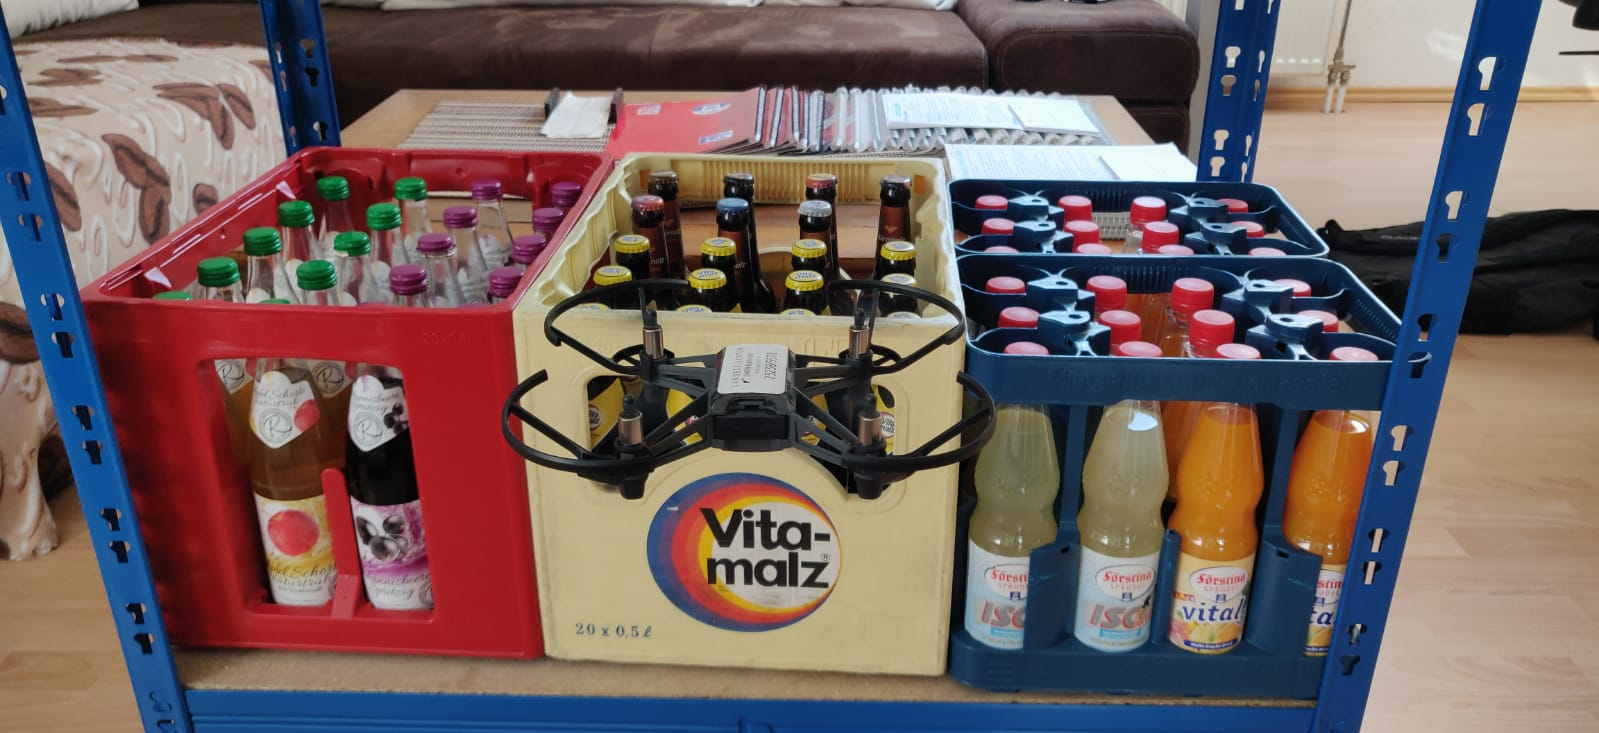
\includegraphics[width=8cm]{Bilder/detail_scan.jpeg}} 
	\subfigure[Drohne während der Gesamtaufnahme]{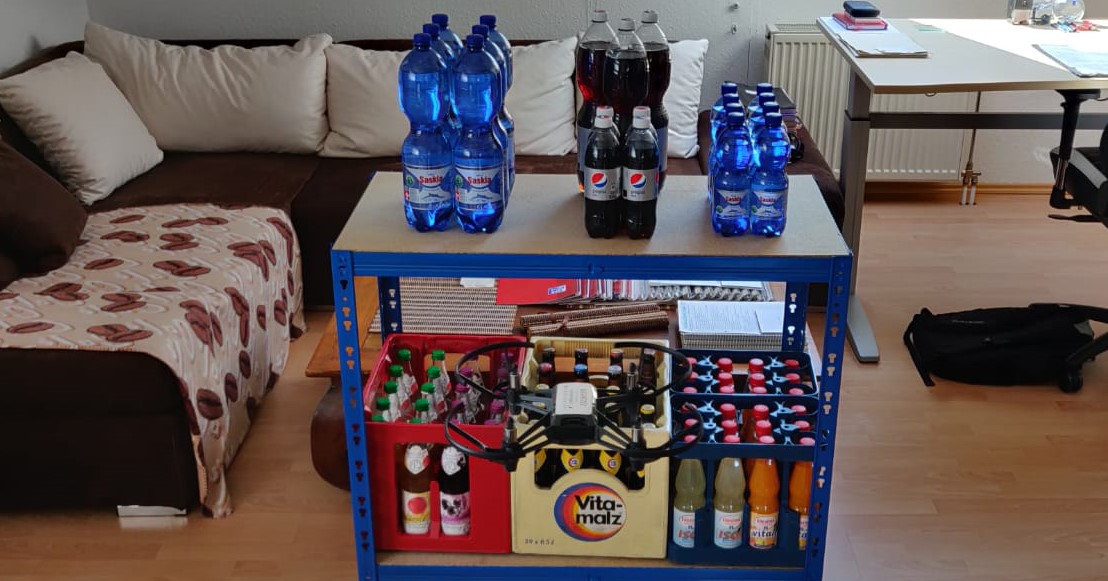
\includegraphics[width=7cm]{Bilder/all_scan.jpeg}} 
	\caption[Drohnenflugsequenz]{Drohnenflugsequenz} 
	\label{sequenz}
\end{figure} 

Mit diesen zwei Methoden wird ein synchroner Versand der Befehle möglich, bei dem immer nur dann ein neuer Befehl geschickt wird, wenn bereits eine Antwort auf den vorherigen empfangen oder ein Timeout erkannt wurde. In der Flugsequenz fliegt die Drohne zunächst nah vor einem Regal mit zwei Böden her, um alle Objekte aus der Nahaufnahme detektieren zu können, danach fliegt die Drohne zurück, um das gesamte Regal im Blickwinkel zu haben (siehe Abbildung \ref{sequenz}). Die finale Befehlskette sieht wie folgt aus:

\begin{itemize}
	\item Command (Übernahme der Steuerung)
	\item streamon (Einschalten von Video Stream)
	\item up 150 (Aufsteigen um 150 cm)
	\item right 100 (Nach rechts fliegen um 100 cm)
	\item down 100 (Absteigen um 100 cm)
	\item left 100 (Nach links fliegen um 100 cm)
	\item up 100 (Nach oben fliegen um 100 cm)
	\item right 50 (Nach rechts fliegen um 50 cm)
	\item back 150 (Nach hinten fliegen um 150 cm)
	\item streamoff (Ausschalten von Video Stream)
	\item land (Landung)
\end{itemize}

Die Befehlssequenz zur Steuerung der Drohne wird parallel zur Inferenz der Bilder ausgeführt, wie durch Abbildung \ref{sequence_diagram} verdeutlicht.

\begin{figure}[H]
	\begin{center}
		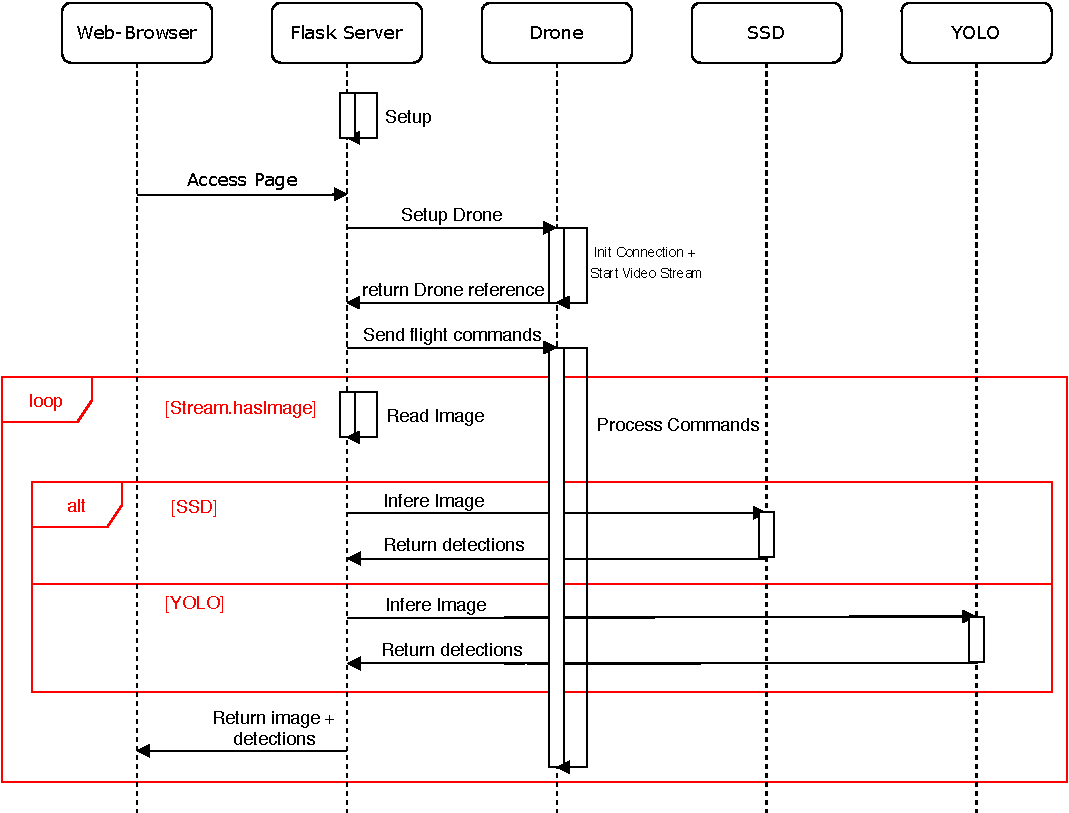
\includegraphics[width=15cm]{Bilder/sequence_diagram.pdf}
		\caption[Ablaufsequenz für die Verarbeitung von Drohnenbefehlen und Inferenz von Bildern]{Ablaufsequenz für die Verarbeitung von Drohnenbefehlen und Inferenz von Bildern}
		\label{sequence_diagram}
	\end{center}
\end{figure}

\subsection*{Modellinferenz}

Der Video Stream der Drohne kann auf dem zentralen Server mittels der \textit{openCV} Klasse \textit{VideoCapture} in Python über das UDP Protokoll angesprochen werden. Anschließend kann jeder Frame des Streams einzeln durch \textit{SSD} inferiert werden.

Da das \textit{Darknet} Framework für \textit{YOLO} allerdings wie zuvor angemerkt in C implementiert ist, kann keine nahtlose Inferenz auf dem Python Server wie bei \textit{SSD} umgesetzt werden. Hierfür muss auf die Kompilierung einer \textit{Dynamic Link Library} (DLL) zurückgegriffen werden. Eine \textit{DLL} ist eine ausführbare Datei, die Funktionen und Ressourcen als geteilte Bibliothek bereitstellt. Programme, die in verschiedenen Programmiersprachen implementiert wurden, können dadurch die gleiche DLL-Funktion aufrufen und die Inferenz mit \textit{YOLO} kann somit durch das Python Programm aufgerufen werden \cite{MicrosoftCorporation.27.01.2020}.
